\begin{frame}[t]
\frametitle{TCF {\small Turbulent Channel Flow}}
\only<1>{
\textbf{Problem setting:}
\begin{itemize}
  	\item Wall bounded flow
    \item $Re_\tau=180$ and $Re_\tau=395$
    \item Mesh resolution: $32^3-Q1$ (stretched elements near the wall)
  \end{itemize}
  \begin{figure}
    \centering	
    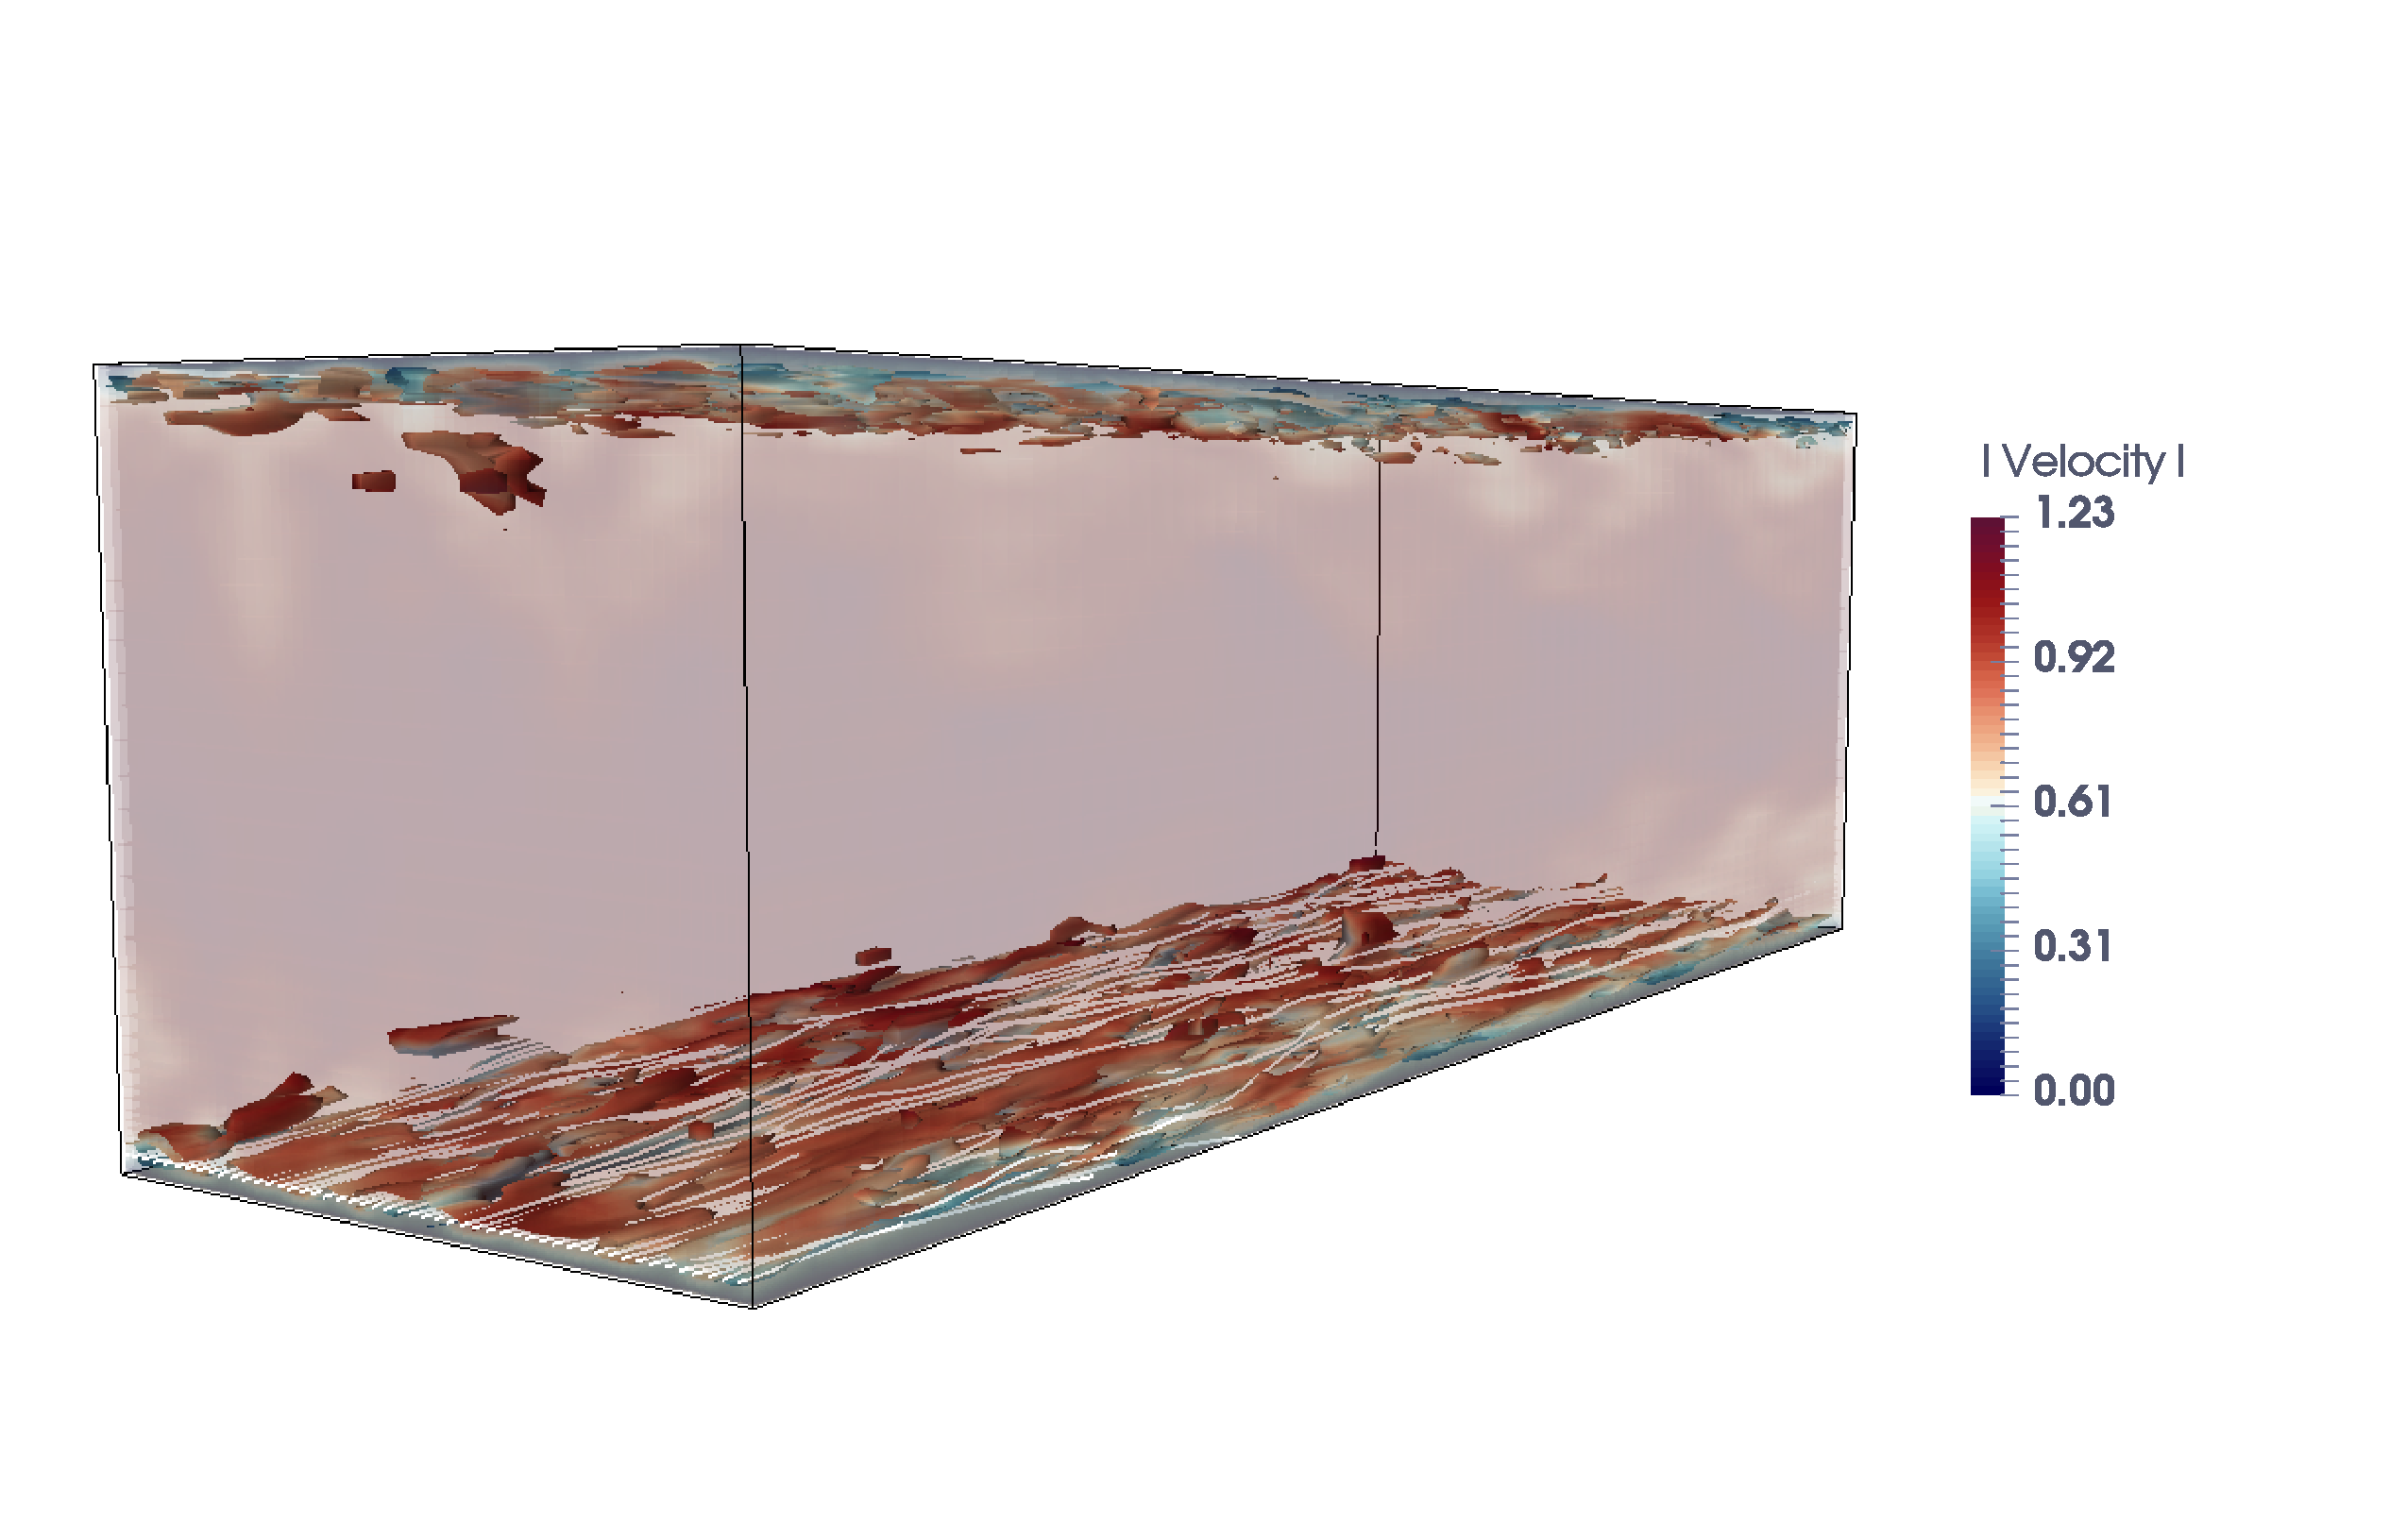
\includegraphics[width=0.8\textwidth,clip=true,trim=0cm 0cm 8cm  5cm]{Figures/cha395_32el_70}
  \end{figure}}
\only<2>{
\begin{figure}[h!]
\centering    
\movie[label=show3,width=1.0\textwidth,poster,autostart,showcontrols,loop]{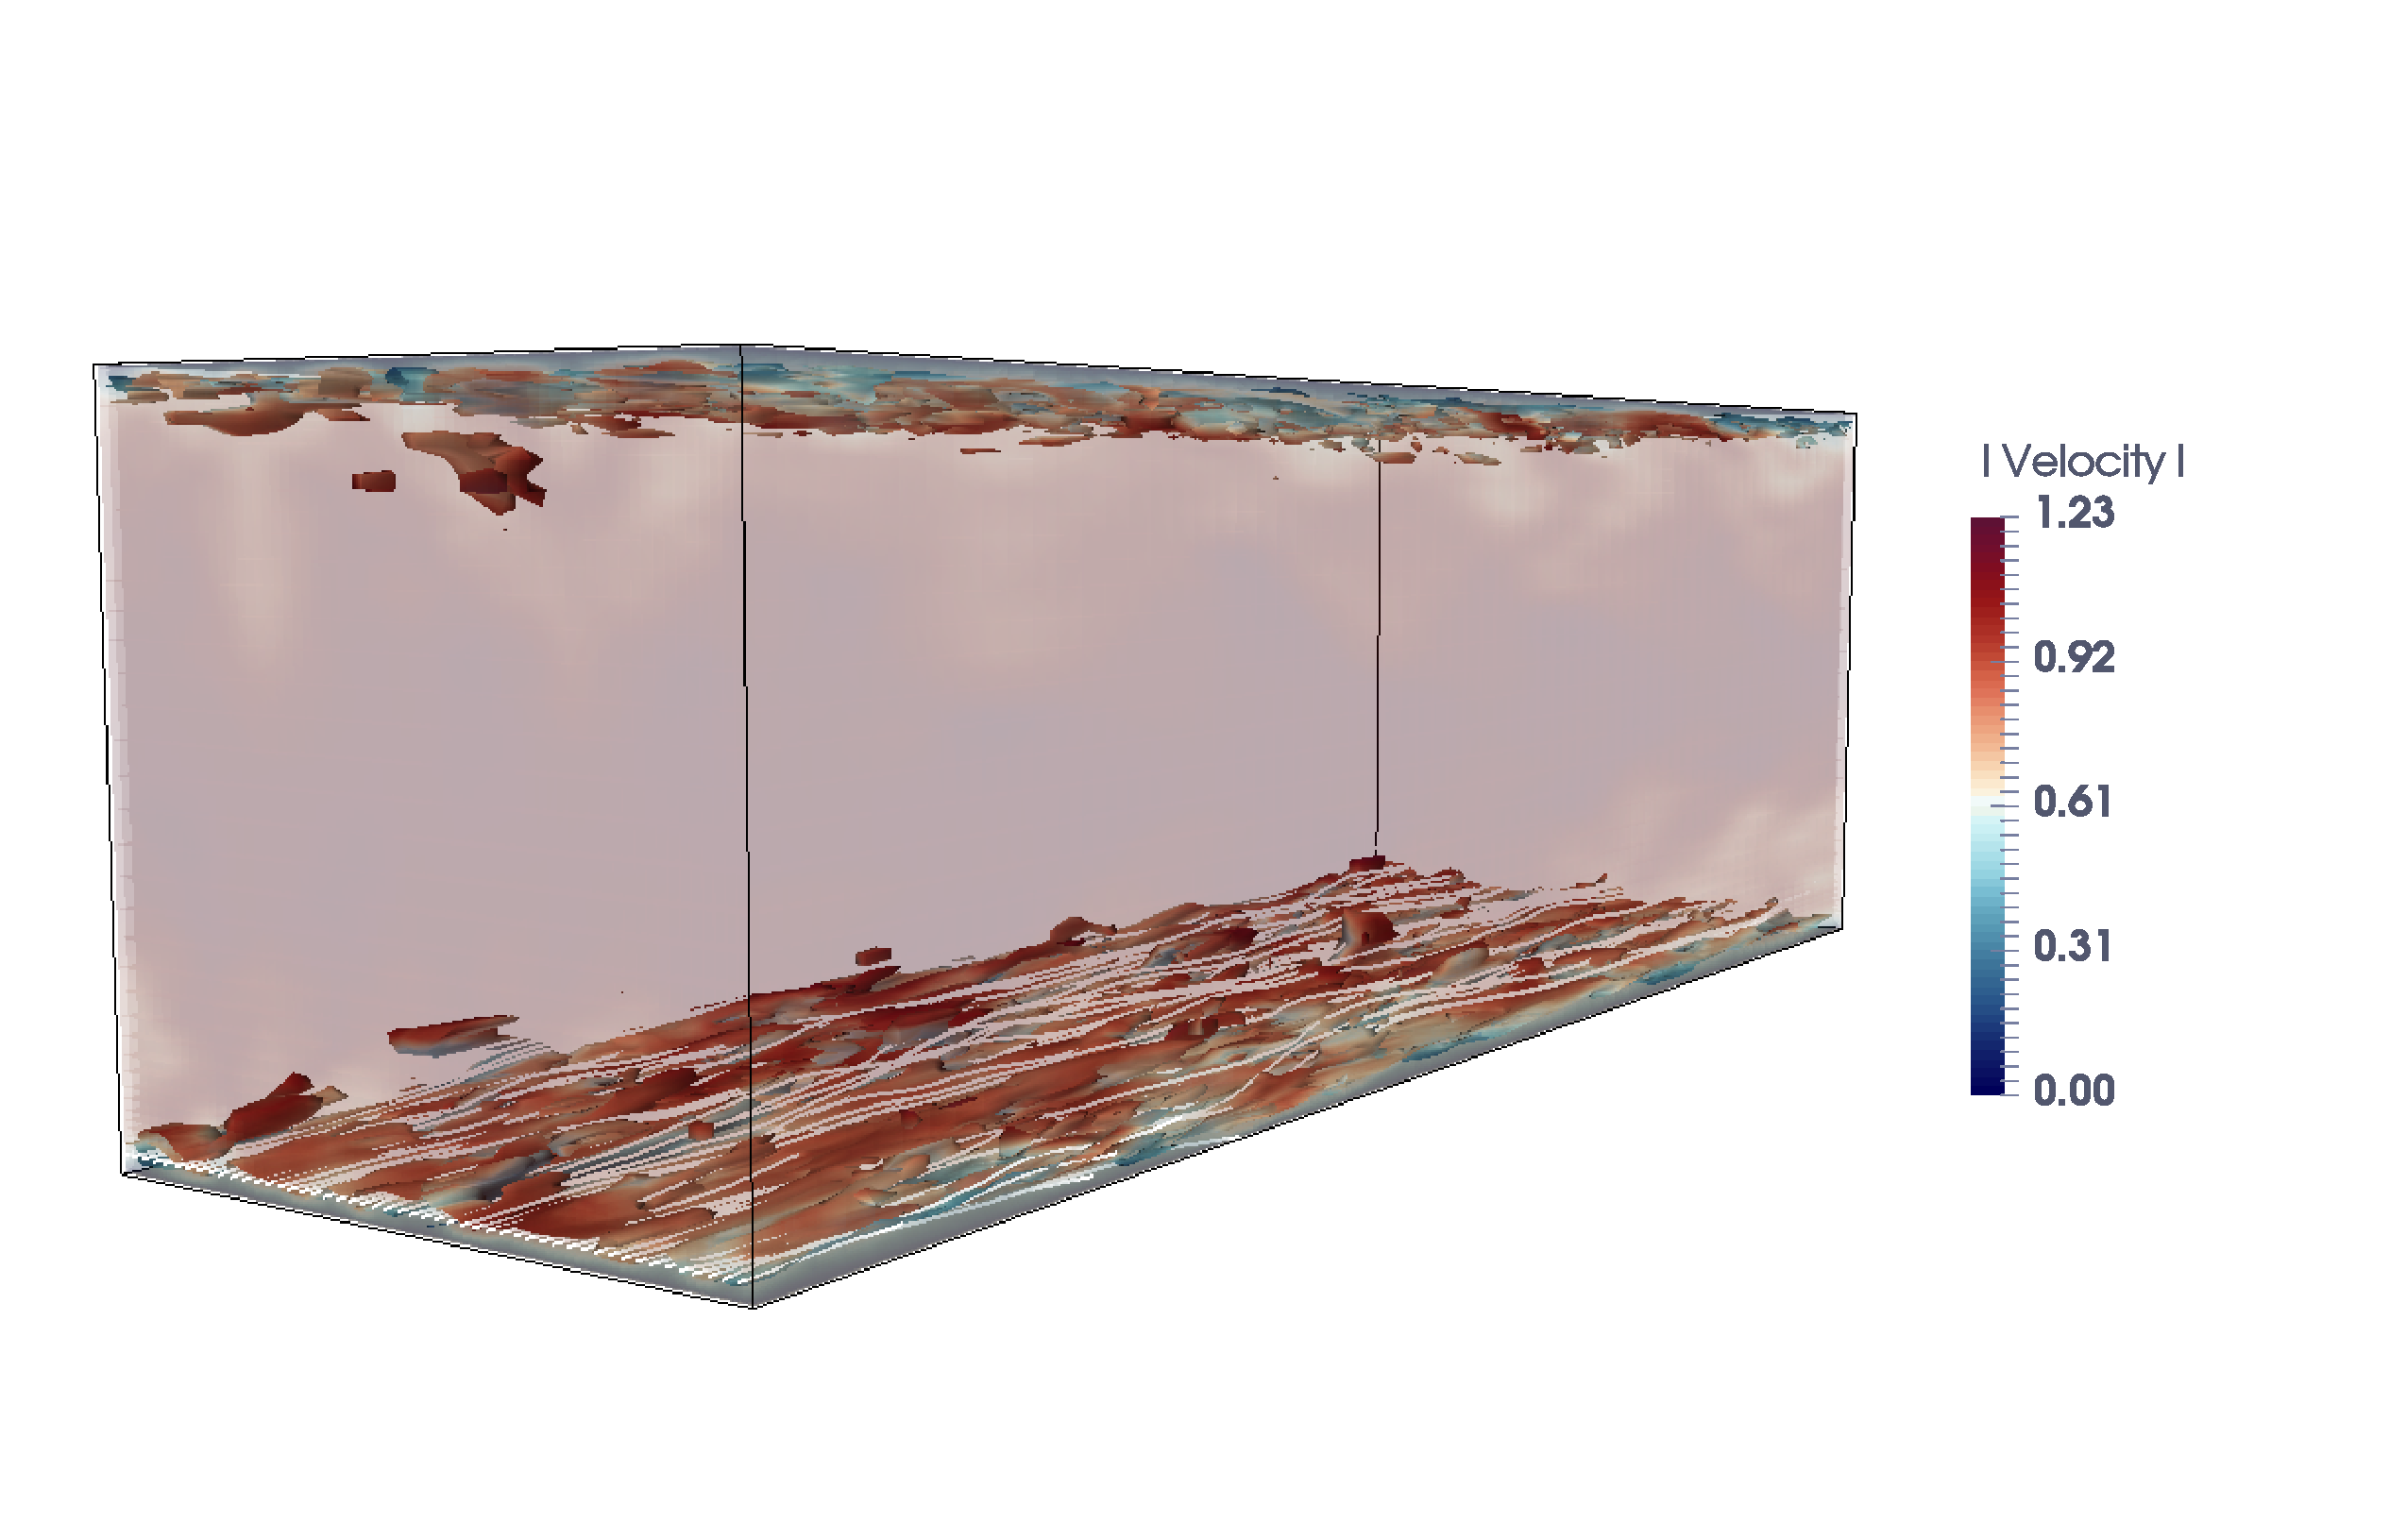
\includegraphics[width=1.0\textwidth]{Figures/cha395_32el_70}}{Movies/TCF.avi}
%\includemedia[activate=onclick,width=1.0\textwidth]{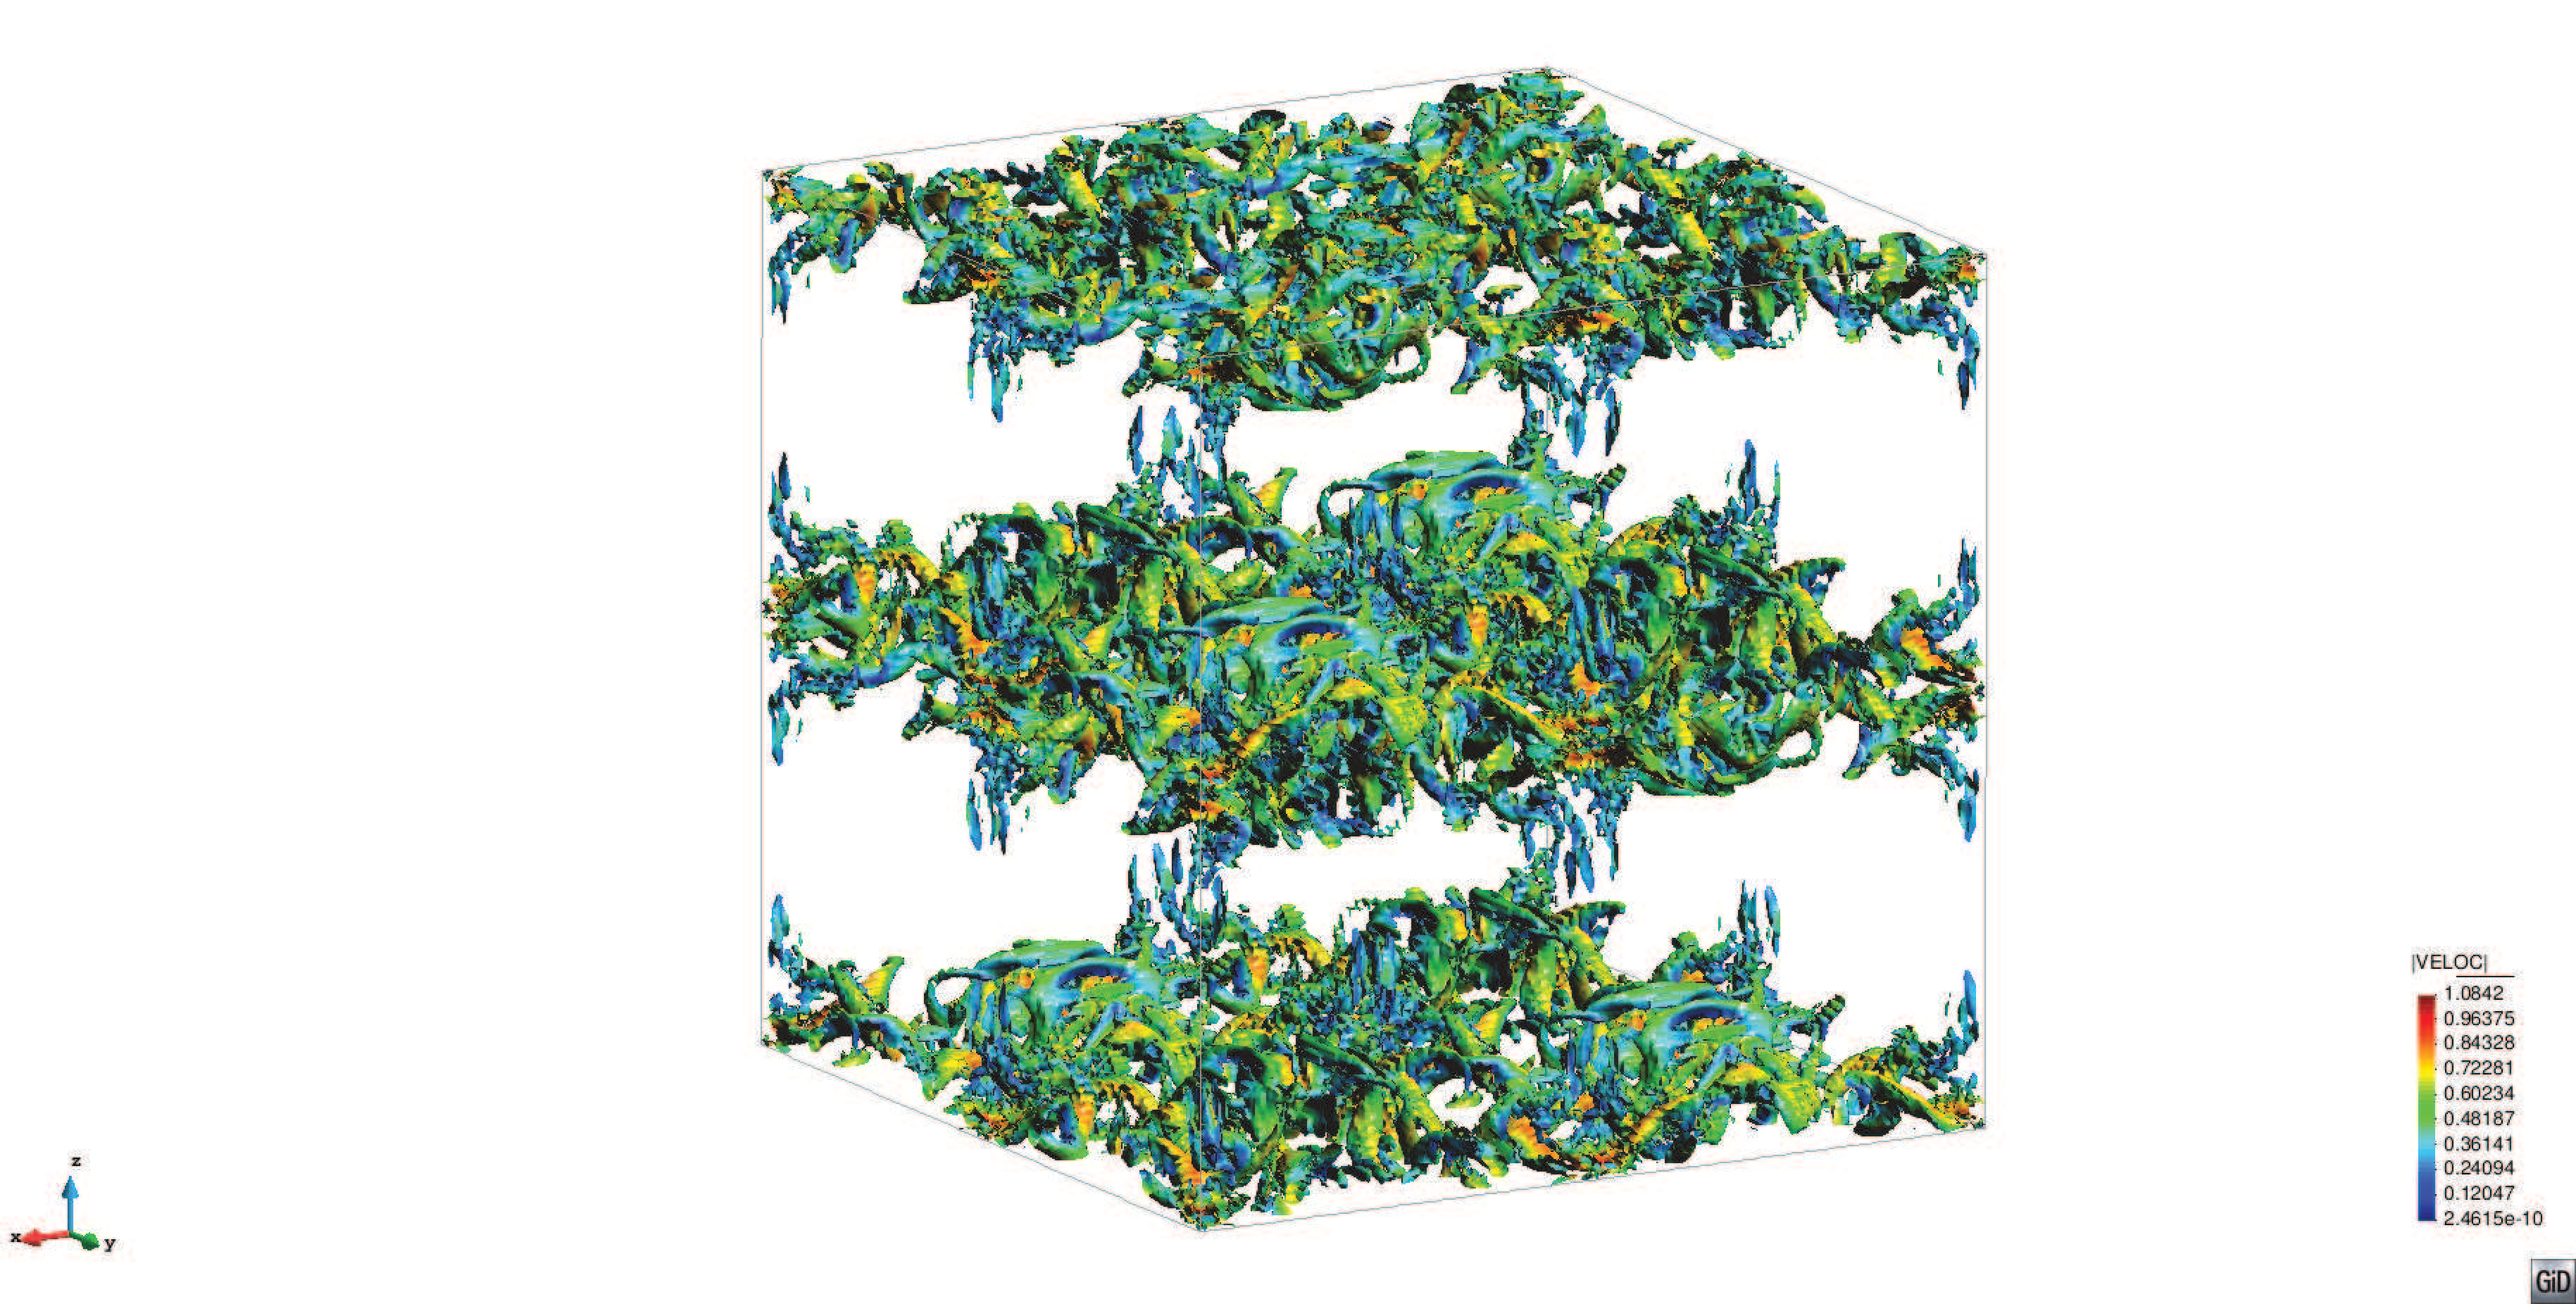
\includegraphics[width=1.0\textwidth]{Figures/isovorti_veloc_6}}{Movies/TGV.flv}
  \caption{Velocity isosurface}
\end{figure}}
\end{frame}
%---------------------------------------------------------------------------
\begin{frame}[t]
\frametitle{TCF {\small Turbulent Channel Flow}}
\textbf{Mean stream-wise velocity (models):}
 \vspace*{-0.3cm}
  \begin{figure}
    \centering	
    \only<1-3>{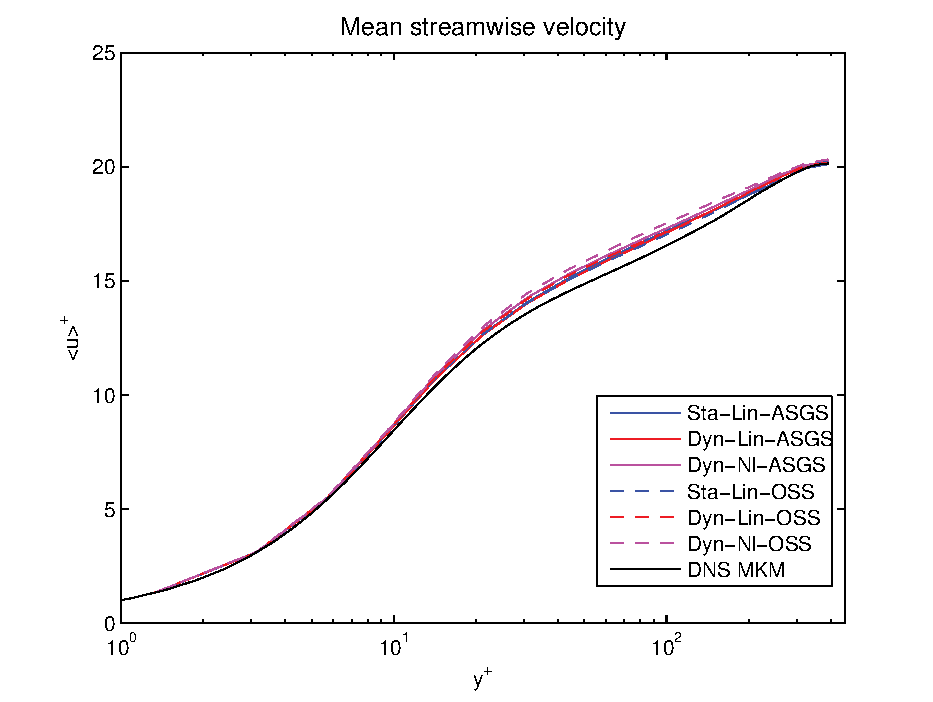
\includegraphics[width=0.65\textwidth]{Figures/Rb_TCF/umean}}
    \only<4>{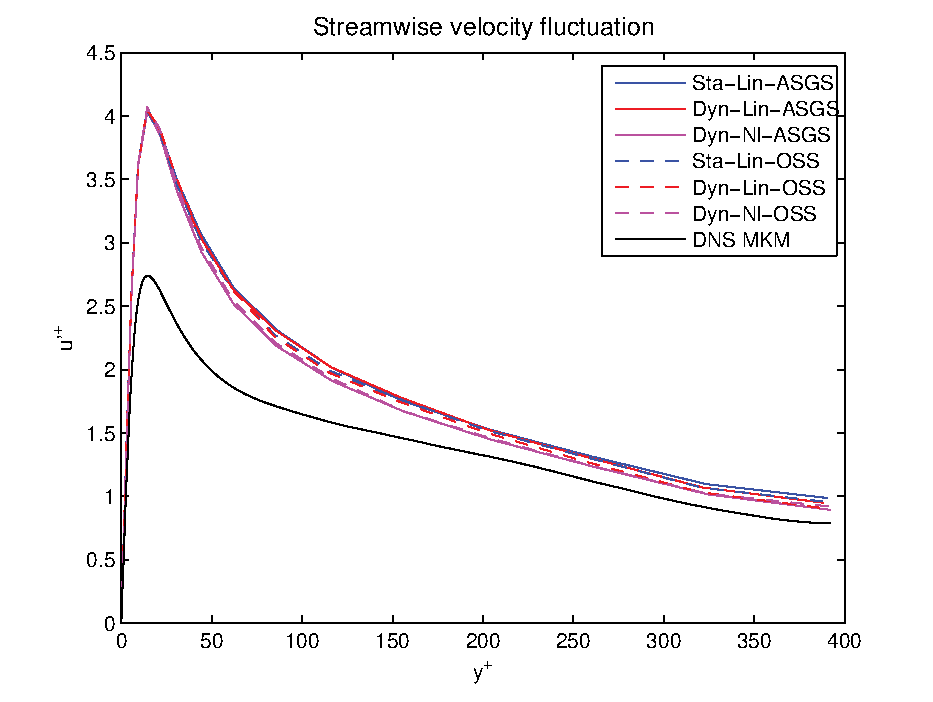
\includegraphics[width=0.65\textwidth]{Figures/Rb_TCF/ufluc}}
    \only<5>{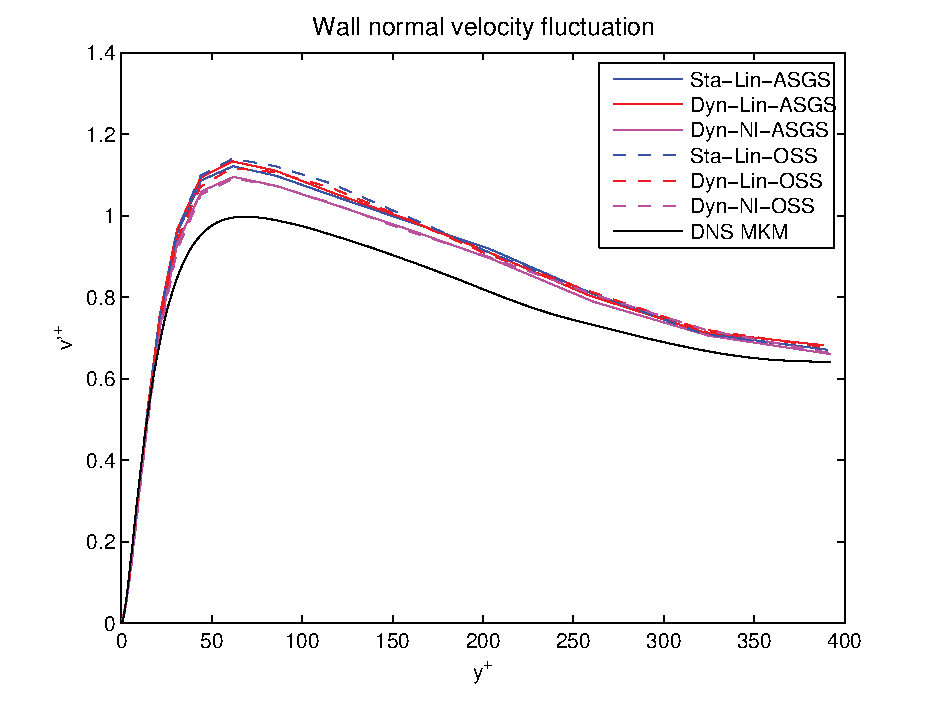
\includegraphics[width=0.65\textwidth]{Figures/Rb_TCF/vfluc}}
    \only<6>{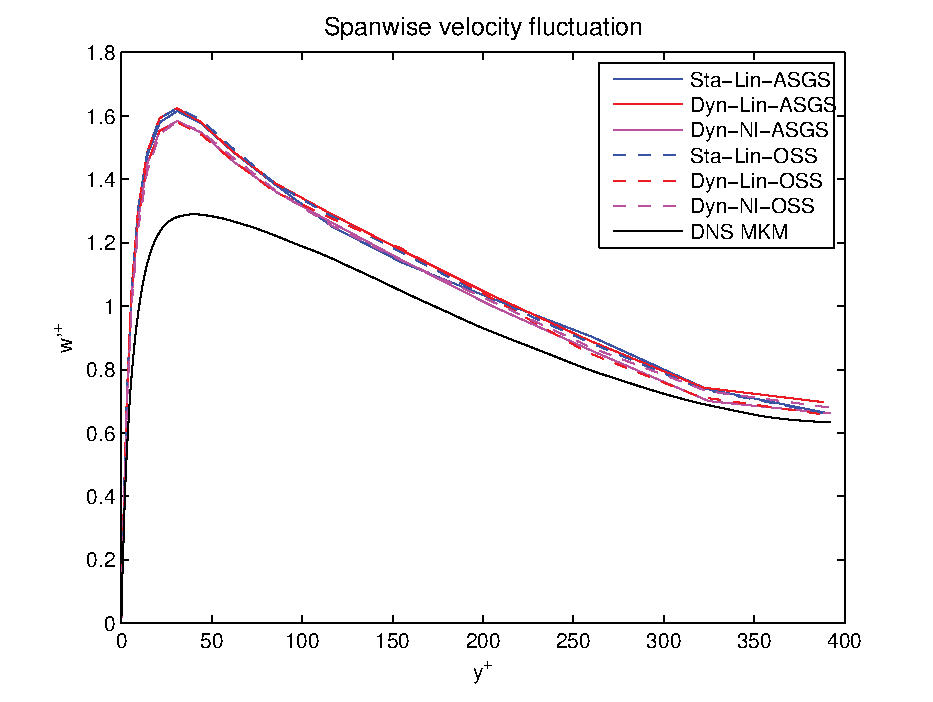
\includegraphics[width=0.65\textwidth]{Figures/Rb_TCF/wfluc}} 
  \end{figure}
  \vspace*{-0.5cm}
   \begin{overlayarea}{\textwidth}{1.5cm}
 \only<2->{
 \begin{itemize}
  	\item \alert<2>{Small differences between methods}
  	\only<3->{\item Very \alert<3>{accurate results} compared against the \alert<3>{DNS}}
  \end{itemize}}
  \end{overlayarea}
\end{frame}